\documentclass[graybox]{svmult}

\usepackage{mathptmx}
\usepackage{helvet}
\usepackage{courier}
\usepackage{type1cm}
\usepackage{makeidx}
\usepackage{graphicx}
\graphicspath{{figures/}}
\usepackage{multicol}
\usepackage[bottom]{footmisc}
\usepackage{amsmath}
\usepackage{amssymb}
\usepackage{url}
\makeindex

% Author-note markers print in bold so they cannot be missed in the proof.
% To hide the two author-note markers once they are filled in, change the line
% below to:  \newcommand{\authornote}[1]{}
\newcommand{\authornote}[1]{\textbf{#1}}

\begin{document}

\title*{Capacity Is Not Access: Agent-Based Modeling of Clean-Air Shelter Siting During Wildfire Smoke in Portland}
\titlerunning{Capacity Is Not Access}
\author{Fatima Asghar}
\authorrunning{Fatima Asghar}
\institute{Fatima Asghar \at Harrisburg University of Science and Technology, Harrisburg, PA, \email{fxa28196@hawkmail.hacc.edu}}
\maketitle

\abstract{Most planning for emergency clean-air shelters uses static screening
maps. Because their inputs are fixed geographic features, these maps cannot show
whether residents can reach a shelter, or what happens when one fills. This study
developed an agent-based model of unsheltered residents moving through Portland's
street network during a smoke event, with individual walking speeds, route choice,
and refusal at full facilities. It contains 6,842 residents, the 2025
Point-in-Time unsheltered count for Multnomah County, each starting at a real
reported campsite and carrying a sampled age, sex, mobility status, and
respiratory health. The smoke is measured, not modeled: hourly readings from the
September 2020 event. Three siting scenarios were compared across nine random
seeds. The present 36-facility system shelters 30.1\% of residents. Raising
capacity to match the population, without moving any facility, shelters 91.6\%
and still refuses 562 people, though the system then holds one space per person.
Spending that identical capacity on ten better-placed sites shelters 96.0\% and
cuts refusals to 256. Equity depends on how the gap is measured; three measures
are reported, and residents with mobility limitations remain the worst-served
group under every scenario. No observational occupancy record could be located,
so these are model-to-model comparisons.}

\section{Introduction}
\label{sec:intro}

In September 2020, wildfire smoke settled over Portland, Oregon for nine days.
Fine particulate matter, the microscopic soot that makes smoke dangerous to
breathe, is measured in micrograms per cubic meter and abbreviated PM$_{2.5}$.
Across the thirteen-day window containing those nine days, it peaked at 562.7
$\mu$g\,m$^{-3}$ and stayed above the U.S. Environmental Protection Agency's
``Unhealthy'' threshold for 194 of 312 hours.

Oregon's Department of Environmental Quality reports that this was Portland's
first experience of air that bad from wildfire. Between 1985 and 2014 the city
recorded no smoke days at or above the ``Unhealthy for Sensitive Groups''
category. In 2020 it recorded three very unhealthy days and five hazardous ones
\cite{deq2023}.

The public health advice during an episode like this is to stay indoors. For
several thousand people in Multnomah County, that advice describes something they
do not have. The county opened clean-air shelters in response to the 2020 event.
This chapter asks what would happen if the same smoke arrived today, measured
against the shelter system that exists now.

Two responses are available, and they are not the same. The county could add
capacity, meaning more spaces inside the buildings it already operates. Or it
could add capacity in better places. These sound like two versions of one idea.
They are not, and the difference matters both for how many people get indoors and
for which people do.

\textbf{Research question.} For a fixed total shelter capacity, does the
geographic placement of that capacity change how many unsheltered residents reach
a clean-air shelter during a smoke episode, and does it change which residents
reach one?

I use an agent-based model because the question is about individuals competing
for a limited resource. A shelter that is full turns away the next person to
arrive. Who arrives first depends on where that person started and how fast they
walk, and how fast they walk depends on their age and their health. None of this
survives being averaged.

A static screening map reports the burden carried by a neighborhood. It cannot
report that 562 people were refused shelter during an event in which the system
held exactly one space per person, which is the central result here.

The model is narrow in what it claims. It measures how much smoke each resident
is exposed to and how much particulate matter each one inhales. It does not
predict illness, hospitalization, or death.

\section{Related Work and Background}
\label{sec:related}

\textbf{Static screening and its limits.} Emergency shelter siting is guided
largely by static screening tools, of which the EPA's EJScreen and California's
CalEnviroScreen are the canonical examples. These combine fixed geographic
features, including land use, population density, poverty rates, and modeled
baseline pollution, into an index that flags high-burden neighborhoods, and
planners place capacity in the flagged areas. This is not a weak comparison. It
is the standard approach and it answers its own question well. The problem comes
when a shelter fills. The people it refuses do not disappear. They keep walking,
or they stop walking, and they keep breathing smoke either way. A static index
cannot show this, because none of its inputs change when a facility reaches
capacity.

\textbf{Agent-based approaches to hazard sheltering.} Siam et al.
\cite{siam2022} build an interdisciplinary agent-based model of wildfire
evacuation that couples fire spread with population response, a transportation
network, and shelter locations, and examine how evacuees' physical
characteristics and travel speed affect who reaches safety. That work addresses
evacuation from an advancing fire, in which the hazard moves and the population
leaves. The problem here differs in kind: the hazard is stationary smoke covering
the whole county for days, nobody leaves, and the binding constraint is a fixed
set of indoor spaces that fill up. The gap addressed here is therefore narrow. It
asks whether modeling residents as individuals who move, queue, and are refused
produces siting conclusions that an index built from fixed geographic features
cannot.

\textbf{Wildfire smoke and health.} Reid et al. \cite{reid2016} find consistent
evidence that wildfire smoke worsens respiratory illness, with weaker evidence
for effects on the heart and circulatory system. DeFlorio-Barker et al.
\cite{deflorio2019} establish that wildfire and non-wildfire particulate exposure
are worth distinguishing. DeVries et al. \cite{devries2017} pool 37 studies
covering roughly 1.1 million emergency events related to chronic obstructive
pulmonary disease, or COPD, and report a 2.5\% increase (95\% confidence interval
1.6\% to 3.4\%) in COPD-related emergency visits and admissions for every
additional 10 $\mu$g\,m$^{-3}$ of PM$_{2.5}$. That figure is easy to misuse. It
describes a relationship between pollution in the air and the COPD emergencies
that follow. It does not describe how much more vulnerable a person with COPD is
than a person without one. Section~\ref{sec:exposure} describes what happened
when I tried to use figures of this kind as exposure multipliers.

\textbf{Health of people experiencing homelessness.} Fazel et al.
\cite{fazel2014} summarize what is known about homeless health in wealthy
countries. For respiratory prevalence the standard national surveys are
structurally unusable here, because they sample from housing units and so exclude
unsheltered people by construction rather than by chance. Zellmer et al.
\cite{zellmer2025} work around this using electronic health records: across
20,139 adults with recent experience of homelessness, diagnosed asthma is 14.9\%
and COPD 10.5\%, against 7.1\% and 3.0\% in a housed comparison group. Brown et
al. \cite{brown2017} found 26.3\% of 350 homeless adults aged 50 and over had
asthma, COPD, or both, essentially identical to the all-ages figure from a large
statewide California study \cite{ucsf2023}. Because the rate among older adults
matches the rate across all ages, I sample respiratory conditions independently
of a resident's age.

\textbf{Movement.} Bohannon and Williams Andrews \cite{bohannon2011} provide
comfortable walking speeds by age decade and sex from a meta-analysis of 41
studies and 23,111 participants, and Bohannon \cite{bohannon1997} supplies a
measure of how much individual speeds vary within a group. For residents with
mobility limitations, Boyce et al. \cite{boyce1999} report movement speeds by
category of impairment, from research on building evacuation. Buekers et al.
\cite{buekers2024} reviewed 25 studies comparing 1,015 people with COPD against
2,229 healthy controls and report that people with COPD walk 19 cm\,s$^{-1}$
slower (95\% confidence interval 11 to 28), rating the evidence low quality. I
searched for an equivalent figure for asthma and did not find one. The literature
supports lower physical activity among adults with asthma, but not a comparable
measurement of walking speed. Section~\ref{sec:equity} reports the consequence as
a finding rather than concealing it.

\textbf{Modeling platform and algorithms.} The model uses Repast Simphony
\cite{north2013}. Routing uses Dijkstra's algorithm \cite{dijkstra1959} over a
map in which each street segment carries its true length on the curved surface of
the earth, computed using Karney's methods \cite{karney2013}. Choosing where to
put new shelters belongs to a class of problems that cannot be solved exactly at
this scale, so I use an approximation method. Section~\ref{sec:scenarios} states
what that method does not guarantee.

\section{Data and Methods}
\label{sec:data}

\subsection{Data Collection}
\label{sec:collection}

Every dataset is recorded in a provenance registry in the project repository,
with its source, web address, retrieval date, license, a cryptographic checksum,
and every transformation applied. A checksum is a short code computed from a
file's contents; if one byte changes, the code changes, which makes it possible
to prove that a result came from exactly the data claimed.
Table~\ref{tab:inputs} summarizes the five inputs.

\begin{table}[t]
\caption{Model inputs. Each row's checksum is recorded in the repository's data
registry and re-verified into every run record, so a result can be tied to the
exact bytes that produced it.}
\label{tab:inputs}
\begin{tabular}{p{2.0cm}p{3.1cm}p{1.8cm}p{3.0cm}}
\hline\noalign{\smallskip}
Dataset & Source & Retrieved & Content \\
\noalign{\smallskip}\svhline\noalign{\smallskip}
Hourly PM$_{2.5}$ & U.S. EPA Air Quality System, parameter 88502 \cite{epaaqs2020} & 2026-07-24 & 4,795 rows; 312 hourly slices, no gaps \\
Street centerlines & Portland Metro RLIS & not recorded & 112,070 polylines; 89,322-node graph \\
Encampment points & City of Portland campsite reports \cite{portlandcampsites} & 2026-07-24 & 3,400 points; 2,981 used \\
Shelter inventory & Multnomah County HSD \cite{multcohsd}; City of Portland \cite{portlandsrv} & 2026-07-24 & 36 facilities, 2,234 spaces \\
Population count & 2025 Tri-County Point-in-Time count \cite{psupit2025} & 2026-07-25 & 6,842 unsheltered \\
\noalign{\smallskip}\hline
\end{tabular}
\end{table}

\subsubsection{The smoke event}
\label{sec:smoke}

The EPA publishes air quality measurements under numbered parameter codes. I use
parameter 88502 rather than the Federal Reference Method series, 88101, because
the 2020 hourly 88101 file contains no monitors in Multnomah County; only Harney,
Klamath, and Lane counties report it in Oregon. Parameter 88502 is what Oregon
DEQ's Portland-area monitors report and what feeds the real-time index the public
sees. The trade-off is that 88502 is approved for index reporting but is not a
reference method.

Filtering the national archive to the three Portland-area counties yields 4,795
hourly records from seven monitors, two of them inside Multnomah County. No value
was altered, rounded, converted, gap-filled, or averaged during extraction, and
the retrieval script reproduces the source file exactly. Averaging the two
in-county monitors hour by hour produces the series in Fig.~\ref{fig:pm25}, which
covers all 312 hours with no missing values. The EPA's own data carries an
informational flag, code IT, meaning ``Wildfire, U.S.,'' on 1,576 records
spanning exactly 7 to 19 September. This is the agency attesting that these
observations were smoke-influenced.

One limitation deserves attention. All seven monitors use a single technique,
heated-inlet nephelometry, so there is no diversity of method and no co-located
reference instrument, and the column recording measurement uncertainty is empty
in all 4,795 records. A heated inlet evaporates semi-volatile organic compounds
before measurement, and those compounds make up a large share of the mass of
fresh wood smoke. These readings most likely understate true PM$_{2.5}$ during
the event.

\begin{figure}[t]
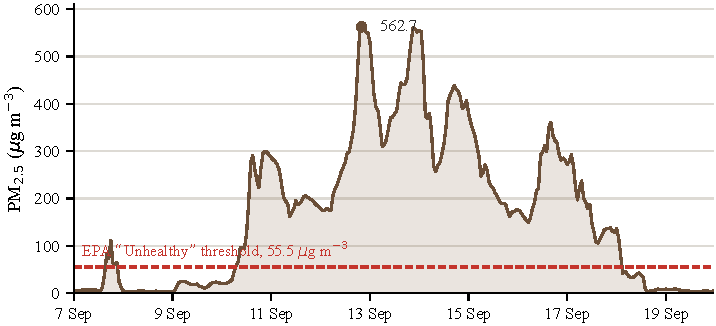
\includegraphics[width=\textwidth]{fig1_pm25}
\caption{Measured hourly PM$_{2.5}$ in Multnomah County, 7--19 September 2020,
averaged across the two in-county regulatory monitors. The air stayed above the
``Unhealthy'' threshold for 194 of 312 hours and peaked at 562.7
$\mu$g\,m$^{-3}$. This drives every result in the chapter. It is measured rather
than modeled, and it is identical in all three scenarios.}
\label{fig:pm25}
\end{figure}

\subsubsection{Where people are}
\label{sec:people}

The count of unsheltered residents comes from the 2025 Tri-County Point-in-Time
count \cite{psupit2025}, a survey conducted on a single night. It recorded 10,526
people experiencing homelessness in Multnomah County, about 65\% of them
unsheltered, which gives 6,842. I use the unsheltered subset rather than the
total, because people already in shelter are indoors and do not walk anywhere in
this model, and the Point-in-Time figure rather than the county's annual service
count of 6,731, because the annual figure counts turnover across a year rather
than people outside on one night. The report's own caution travels with the
number: changes in how administrative data were incorporated substantially
increased the 2025 unsheltered count, so the comparison from 2019 to 2025 is not
a clean time series and is not presented as one.

Residents start at real locations. The City of Portland publishes campsite
reports through its Impact Reduction Program, and 3,400 were retrieved through
the city's open data service \cite{portlandcampsites}; the runs reported here
place residents at 2,981 distinct locations. Two limitations matter. The feed
covers only a recent rolling window and retains no records from 2020, so 2025 and
2026 locations serve as a geographic stand-in for the 2020 distribution, and the
model prints a warning to this effect at the start of every run. The reports are
also generated by public complaints, which biases them toward camps visible from
the street.

\subsubsection{Where the shelters are, and the street network}
\label{sec:shelters}

The county's published shelter list \cite{multcohsd} mixes five incompatible
units: beds, motel rooms, village units and pods, family units, and counts with
no stated unit. It cannot be added up directly. I converted each unit into people
using explicit ranges rather than single values. A bed holds one person. A motel
room serving ``individuals and couples'' holds 1.0 to 1.5. A village unit holds
1.0 to 1.2. A family unit holds 2.5 to 4.0, and is the weakest conversion in the
set. A count with no stated unit is treated as a count of people, which is the
most conservative reading, because it cannot inflate the total. Applying the
midpoint of each range across the 36 clean-air-capable facilities gives a modeled
total of 2,234 spaces.

No coordinate was guessed. The raw inventory file contains no coordinates, so
every location was geocoded from a published street address, with each record
noting which service produced the coordinate and at what confidence. Six
addresses for City Safe Rest Villages were recovered from municipal
announcements \cite{portlandsrv}. Three of the 36 coordinates resolve only to a
block or an intersection: the geocoding service refuses intersection queries, so
I resolved those to the corresponding hundred-block address, an approximation of
a few hundred meters recorded as such in the confidence column rather than
presented as a precise address. The other 33 are full street addresses.

Two facilities are excluded because neither publishes a street address: Clinton
Triangle, which at 160 units is the largest single site in the inventory, and
Multnomah Safe Rest Village at 28. Real capacity is therefore roughly 207 people
higher than modeled. Ten day centers are also excluded because none publishes a
capacity.

Street centerlines come from Portland Metro's Regional Land Information System
and are redistributed as received. This is the one input whose retrieval date was
not recorded and whose original release version and license could not be
recovered; the repository states its terms as unverified rather than relicensing
it.

\subsection{Methods}
\label{sec:methods}

\subsubsection{Platform, languages, and tools}
\label{sec:platform}

The simulation is written in Java 17 on Repast Simphony 2.11 \cite{north2013},
built with Gradle, and uses the GeographicLib library for distances on the curved
surface of the earth and the JTS Topology Suite for spatial indexing. Analysis,
figure generation, scenario construction, and the placement optimizer are Python
3.14 using pandas and Matplotlib. All source, data, configuration, and run
records are in the repository named in the code availability note.

\subsubsection{Agents}
\label{sec:agents}

Each resident is an agent with a state, a position, a starting location, a
walking speed, and a set of sampled attributes. A resident can be waiting to
leave, walking, sheltered, unable to reach any shelter, or turned away because
every shelter within reach was full.

A resident begins in the waiting state at their campsite and departs only when
both conditions in Eq.~\ref{eq:depart} hold at once:

\begin{equation}
\label{eq:depart}
C(t) \ge 55.5\ \mu\mathrm{g}\,\mathrm{m}^{-3}
\quad \wedge \quad
\exists\, s \in S : \mathrm{open}(s,t)
\end{equation}

where $C(t)$ is the countywide PM$_{2.5}$ concentration at hour $t$ and $S$ is
the shelter set. The threshold is the lower boundary of the EPA's ``Unhealthy''
category \cite{epaaqi2024}. I chose this boundary because it is unchanged across
both the pre-2024 and post-2024 breakpoint tables, unlike the boundaries above
it, which were revised. One point about terminology: the EPA's categories are
defined on 24-hour averages while this model counts hourly observations, so I
never describe a result as falling in an index category. The derived measure is
named and defined as hours above a stated concentration.

Attributes are drawn from the sources in Table~\ref{tab:attributes}. One
engineering detail matters. Repast shuffles the order in which agents act each
time step, using the same stream of random numbers that assigns each resident to
a campsite, so drawing even one additional number from that stream would silently
change the entire population. The attribute sampler therefore uses a private
stream derived from the run's seed by the formula
$(\mathrm{seed} \times 1000003) + 17$. The verified consequence is that adding
the entire attribute layer left the archived baseline run byte-for-byte
identical.

\begin{table}[t]
\caption{Sampled resident attributes with their sources and realized marginals at
seed 42. Values are either measured from local administrative data (M) or taken
from published literature (L), and the local sources are documented in full, with
retrieval dates and checksums, in the repository's provenance registry. The
asthma target is the Zellmer et al. figure of 14.9\% rounded to 15.0.}
\label{tab:attributes}
\begin{tabular}{p{2.5cm}p{2.3cm}p{2.3cm}p{2.8cm}}
\hline\noalign{\smallskip}
Attribute & Target & Realized & Source \\
\noalign{\smallskip}\svhline\noalign{\smallskip}
Age 18--44 / 45--64 / 65+ (\%) & 52.7 / 42.3 / 5.0 & 52.8 / 42.0 / 5.2 & Pathways Study 2026, $N = 541$, local (M) \authornote{[Pathways Study 2026 - full citation to be confirmed]} \\
Sex M / F / other (\%) & 68.4 / 29.3 / 2.3 & 68.6 / 29.2 / 2.2 & 2019 Multnomah PIT (M) \\
Mobility limitation (\%) & 19.2 & 19.9 & 2019 PIT; a lower bound (M) \\
Asthma (\%) & 15.0 & 14.8 & Zellmer et al. \cite{zellmer2025} (L) \\
COPD (\%) & 10.5 & 10.8 & Zellmer et al. \cite{zellmer2025} (L) \\
Chronic physical condition (\%) & 39.1 & 39.6 & Pathways 2026, local (M) \\
Walking speed (m\,s$^{-1}$) & --- & 1.28 mean & Bohannon and Williams Andrews \cite{bohannon2011} (L) \\
\noalign{\smallskip}\hline
\end{tabular}
\end{table}

\subsubsection{Walking speed}
\label{sec:speed}

Walking speed is the only attribute permitted to change an outcome. Every other
attribute is a reporting category, not a lever.

A resident with no mobility limitation draws a speed from a bell curve centered
on the published average for their age decade and sex, with a standard deviation
of 13\% of that average, taken from Bohannon's measure of within-group variation.
Residents aged 18 and 19 draw from the youngest published stratum, 20 to 29,
because no reference values exist below that age. A resident with COPD has that
average shifted down by 0.19 m\,s$^{-1}$, matching how Buekers et al. report the
difference. A resident with a mobility limitation instead draws from a separate
distribution centered on 0.95 m\,s$^{-1}$ with a standard deviation of 0.32,
which spans the range of Boyce et al.'s impairment categories; this replaces the
age-and-sex average rather than adjusting it, and the COPD reduction is not
applied on top, because the impaired-movement categories already describe a
slower walker. In both cases the speed is truncated to the range 0.4 to 2.2
m\,s$^{-1}$, which excludes implausible values:

\begin{equation}
\label{eq:speed}
v_i \sim
\begin{cases}
\mathcal{N}_{[0.4,\,2.2]}(0.95,\ 0.32) & \text{if mobility limited} \\[4pt]
\mathcal{N}_{[0.4,\,2.2]}\!\left(\mu_{a,s} - 0.19\,\delta_i^{\mathrm{COPD}},\ 0.13\,\mu_{a,s}\right) & \text{otherwise}
\end{cases}
\end{equation}

where $\mu_{a,s}$ is the published mean for age decade $a$ and sex $s$, and
$\delta_i^{\mathrm{COPD}} \in \{0, 1\}$.

The width never comes from the confidence intervals in the 2011 meta-analysis.
Those intervals describe uncertainty about a group average across studies, not
the spread among individuals, and using them would understate the true variation
between people by a factor of three to five. Fig.~\ref{fig:speeds} shows the
resulting distributions.

\begin{figure}[t]
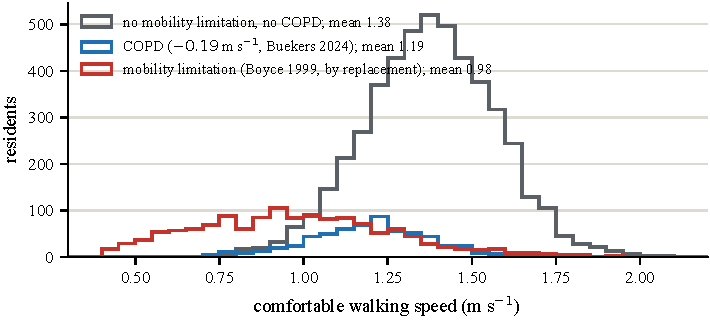
\includegraphics[width=\textwidth]{fig2_speeds}
\caption{Sampled comfortable walking speeds by group. The mobility-limited
distribution (mean 0.98) replaces the age-by-sex distribution (mean 1.38) rather
than rescaling it; the COPD group has mean 1.19. Asthma appears in no group here,
because no published gait-speed decrement exists for it. That absence propagates
directly into the equity result in Sect.~\ref{sec:equity}.}
\label{fig:speeds}
\end{figure}

\subsubsection{Movement and routing}
\label{sec:movement}

The street map becomes a network of 89,322 intersections and 112,070 segments,
each carrying its true length along the curve of the earth \cite{karney2013}. The
map file's own length field is deliberately ignored, because its units are
undocumented.

At setup the model computes one shortest-path tree per shelter, working out in
advance the shortest route from every intersection in the city. Because the
network can be traveled in either direction, the distance from any resident to
any shelter is then a single lookup. This is what allows a 312-hour run of 6,842
residents to finish in under a minute. Each time step, a resident receives a
travel budget equal to their speed times the length of the step and walks that
far along their route, with partial segments finished by an exact geographic
calculation, so movement follows the street network along its true curved length
rather than cutting across in a straight line.

\textbf{A defect in the street data.} During validation I found 27 intersection
identifiers each claimed by two or more different street features, at locations 9
to 18.5 km apart. The map file contains no legitimately multi-part shapes, so
this was an error in labeling rather than a feature of the geography, and the
effect was severe: the affected segments were labeled as a few meters long but
spanned kilometers, so the shortest-path search treated them as cheap shortcuts.
In a fifty-agent test run, 22 of the 50 residents had corrupted journeys, with
travel distances up to 15 times too large, inhaled doses three times too large,
and in some cases a different shelter chosen.

I corrected this without deleting any data. Separating duplicate identifiers that
genuinely describe the same junction from those that describe different places is
straightforward, because a wide empty band divides the two populations: genuine
scatter between the endpoints of connecting streets is under a meter, while the
smallest corrupt displacement is about 1.65 km, and any separating distance
chosen between those two regimes produces an identical corrected network. Every
duplicate claim beyond the first was therefore either reattached to a genuinely
coincident junction, covering 4 cases, or assigned a newly created intersection
at its true location, covering the remaining 23. After correction, the number of
segments whose stated length was inconsistent with the distance between their
endpoints fell from 50 to zero, the largest endpoint gap fell from 18.5 km to
11.9 m, and the connectivity of the network was unchanged. Every correction is
written into the run record.

\subsubsection{Exposure, dose, and the removed risk weighting}
\label{sec:exposure}

The model computes three related quantities and keeps them separate. Exposure is
a property of the air, the total pollution a resident is surrounded by over time:

\begin{equation}
\label{eq:exposure}
E_i = \sum_t C(t)\, \Delta t
\qquad [\mu\mathrm{g}\,\mathrm{m}^{-3}\,\mathrm{h}]
\end{equation}

Inhaled dose is a property of the person. It differs from exposure only by
breathing rate, which here depends on activity and nothing else:

\begin{equation}
\label{eq:dose}
D_i = \sum_t C(t)\, \mathrm{IR}(\alpha_i(t))\, \Delta t,
\quad
\mathrm{IR} =
\begin{cases}
1.62\ \mathrm{m}^{3}\,\mathrm{h}^{-1} & \text{if walking} \\[2pt]
0.61\ \mathrm{m}^{3}\,\mathrm{h}^{-1} & \text{otherwise}
\end{cases}
\end{equation}

with rates from the EPA Exposure Factors Handbook \cite{epaefh2011}. Health risk
is a third quantity, $R_i = D_i \cdot w_i$, where $w_i$ is a susceptibility
weight. In this model $w_i = 1.0$ for every resident, by design. Accumulation
stops when a resident is admitted; residents who are walking, stranded, or turned
away are all still outdoors and keep accumulating.

The reason that weight is inert deserves a full account, because it is the
largest change I made to this project as originally designed. The project was
proposed with a second question alongside the siting question: whether the
recommended placement changes when exposure is weighted by residents' published
age-specific and disease-specific relative risks. This chapter does not answer
that question.

The original design specified two weights: 1.45 for adults aged 65 and over,
attributed to Di et al. \cite{di2017}, and 1.80 for COPD, attributed to a paper
described as ``Anderson et al. 2013.'' Checking both against the publisher
records revealed three problems. First, Di et al. is a real and excellent study
of 60.9 million Medicare beneficiaries, but it reports a hazard ratio of 1.073
per 10 $\mu$g\,m$^{-3}$ of annual PM$_{2.5}$, not 1.45; more fundamentally, every
person in that study is aged 65 or over, so the design cannot produce a
comparison between older and younger adults at all. Second, no paper matching
``Anderson et al. 2013'' with that finding exists. The nearest record is a 2013
study whose first author is Atkinson \cite{atkinson2013}, published in a
different journal, examining cardiovascular disease incidence rather than
respiratory illness, and reporting no COPD effect-modification estimate. Third,
and independently of whether the citations were correct, multiplying an exposure
by a relative risk is a category error. A relative risk is a ratio between the
rates at which an outcome occurs in two groups. It is not a multiplier that can
be applied to an exposure. The correct object would be a ratio between
exposure-response coefficients, which is a different quantity, and the same
underlying data can be made to yield age multipliers differing by more than a
factor of two depending only on which scale is chosen.

I therefore set all susceptibility weights to 1.0 and made group-stratified
reporting the primary way this chapter addresses equity. Outcomes are reported
for each group separately rather than combined into a weighted index that no
source can justify. The weighting slot remains in the code, so a properly sourced
coefficient would have exactly one place to go, and so a reader can see that the
weighting is switched off rather than absent. For the same reason, breathing rate
is held constant across health status: I identified no defensible
population-specific breathing-rate multiplier for walking adults with asthma or
COPD, and any figure I supplied would have been an assumption wearing a citation.

\subsubsection{The three scenarios and experimental design}
\label{sec:scenarios}

The scenarios are not three guesses. Each answers the question the previous one
raised. Scenario A is a measurement rather than a treatment; its only job is to
reveal which constraint binds. It showed that capacity binds, so B relieves
capacity and changes nothing else. B then revealed a further constraint, so C
spends identical capacity differently.

\begin{itemize}
\item \textbf{A, today.} All 36 clean-air-capable facilities at their real
geocoded coordinates with their real capacities: 2,234 spaces.
\item \textbf{B, capacity meets demand.} Every real facility scaled by
$6842/2234 = 3.0627$, rounded so the system total is exactly 6,842. Coordinates,
facility count, and relative facility size unchanged.
\item \textbf{C, the same capacity, better placed.} Real facilities grow by only
1.5$\times$. The remaining capacity becomes ten new facilities at algorithmically
chosen street-network nodes. Total capacity is held identical to B at 6,842.
\end{itemize}

Because B and C hold total capacity exactly equal, a difference between them
isolates where the additional capacity sits and nothing else. C never moves an
existing facility. All 36 stay at their real coordinates, because a real shelter
system cannot be picked up and set down elsewhere.

The ten new locations come from a capacitated greedy \emph{p}-median procedure
over candidate street nodes thinned to one per 600 m grid cell. The objective
minimizes network distance times residents served, plus a declared penalty per
unfilled space; facilities are placed largest-first and served demand is
decremented before the next placement. This is a heuristic, and because shelter
catchments overlap it carries no formal guarantee of near-optimality. The result
is a good placement, not a provably optimal one. The 1.5$\times$ factor and the
choice of ten sites are policy parameters I selected, not measured quantities.

Everything except the shelter file is held identical across scenarios: the same
6,842 residents with the same identifiers, start coordinates, ages, sexes,
mobility statuses, respiratory conditions, and walking speeds; the same smoke
measurements; the same street graph; the same parameters. Each scenario was run
with nine random seeds, 42 through 50, giving 27 runs. Changing the seed changes
which residents receive which attributes while leaving the population
distribution the same. Every result below is from seed 42, with the range across
all nine seeds alongside.

\section{Results}
\label{sec:results}

\subsection{Verification}
\label{sec:verification}

Before reporting outcomes I report what was checked. Several of these tests have
answers that can be worked out by hand, which makes them independent of the
simulation.

The exposure calculation was recomputed in Python directly from the raw EPA file,
outside the model. A resident who never reaches shelter should accumulate the
full-window total of 54,002.7 $\mu$g\,m$^{-3}$\,h; the model reports 54,002.8.
The same residents show a mean concentration of 173.09 $\mu$g\,m$^{-3}$, a peak
of 562.7, and 194.0 hours above threshold, each matching the independently
computed value exactly. Routing was validated against a separate Python
implementation of Dijkstra's algorithm over the same graph, which reproduced the
Java distances exactly across five tests. Rerunning at seed 42 reproduces the
output bit for bit.

One defect motivated a further check. A resident turned away at a full shelter
originally re-planned its route from its immutable start node, meaning it walked
back to its campsite before setting out again, inflating both distance and dose.
The bug was invisible at the fifty-agent test scale because no shelter ever
filled there. After the fix, every run is checked against walked $\le$ planned
$+$ snap gap $+$ 200 m, where the snap gap is the distance from a resident's
start coordinate to its nearest graph node. In a reference run where 250 of 400
residents were refused at least once, the largest unexplained distance was 8.9 m.

Across the 27 production runs, six checks hold every time: the seed and scenario
code in each run manifest match the run performed; the working tree was clean for
every run; the data version is identical across all nine seeds within each
scenario; the set of source file checksums is identical across all 27 runs; each
run exports exactly 6,842 resident records; and within each seed the population
is byte-identical across scenarios, verified by SHA-256 over the joined attribute
vector.

\subsection{Access}
\label{sec:access}

Table~\ref{tab:outcomes} gives the headline outcomes and Fig.~\ref{fig:access}(a)
shows the access result.

Today's system shelters 2,060 of 6,842 residents, or 30.1\%. Capacity binds hard:
4,766 residents are turned away because every facility they can reach is full,
and 33 of the 36 facilities finish the event at capacity. Raising capacity to
meet demand at the same locations lifts this to 6,264, or 91.6\%, a factor of
3.04. Total modeled exposure falls 87.3\% and mean walking distance falls 56.5\%.

One caution about how these numbers should be read. This chapter reports four
exposure measures --- total modeled exposure, mean hours above threshold, mean
inhaled dose, and person-hours above threshold --- and they fall by 87.3\%,
87.1\%, 87.1\%, and 86.9\%. These are not four independent confirmations of one
result. Because the PM$_{2.5}$ field is spatially uniform in this model, all four
are time spent outdoors multiplied by a constant, so they must move together.
They are reported separately because different audiences use different units, not
because they provide separate evidence.

\begin{table}[t]
\caption{Outcomes at seed 42, with the range across all nine seeds in brackets.
No range overlaps between scenarios on any metric. B and C hold identical total
capacity, so the B$\rightarrow$C difference is attributable to placement alone.
The four exposure measures are not independent; see the text.}
\label{tab:outcomes}
\begin{tabular}{p{3.6cm}p{2.1cm}p{2.1cm}p{2.1cm}}
\hline\noalign{\smallskip}
 & A: today & B: more capacity & C: better placed \\
\noalign{\smallskip}\svhline\noalign{\smallskip}
Facilities & 36 & 36 & 46 \\
Total spaces & 2,234 & 6,842 & 6,842 \\
Sheltered & 2,060 (30.1\%) & 6,264 (91.6\%) & 6,570 (96.0\%) \\
range, 9 seeds & [2,053--2,064] & [6,257--6,268] & [6,563--6,574] \\
Turned away, all full & 4,766 & 562 & 256 \\
Spaces left empty & 174 & 578 & 272 \\
No shelter reachable & 16 & 16 & 16 \\
Mean distance walked (m) & 18,260 & 7,938 & 5,689 \\
Mean hours above threshold & 135.8 & 17.5 & 8.6 \\
Mean inhaled dose ($\mu$g) & 23,374 & 3,056 & 1,534 \\
Person-hours above threshold & 928,934 & 119,921 & 59,060 \\
\noalign{\smallskip}\hline
\end{tabular}
\end{table}

\begin{figure}[t]
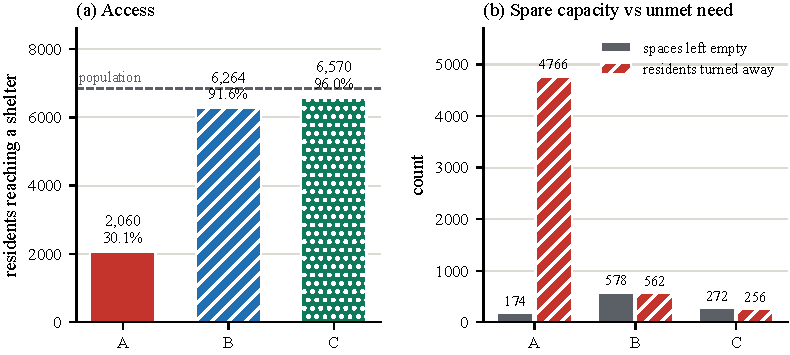
\includegraphics[width=\textwidth]{fig3_access}
\caption{Access outcomes for the three scenarios: (a) residents reaching a
shelter, and (b) spare capacity and unmet need in the same run. Under scenario B
the system holds exactly one space per person and still refuses 562 people,
because the spaces are where the buildings are rather than where the people are.
The equality of empty spaces and unsheltered residents in panel (b) follows from
capacity equaling population; see the text.}
\label{fig:access}
\end{figure}

\subsection{The geography failure}
\label{sec:geography}

Under scenario B the system holds 6,842 spaces for 6,842 residents, exactly one
space per person. It still refuses 562 people.

That is the finding, and it needs stating carefully, because a related
observation is not evidence at all. Scenario B leaves 578 spaces empty and fails
to shelter 578 people, of whom 562 were refused at a full facility and 16 could
reach no facility. Those totals are equal by arithmetic, not by discovery: when
capacity equals population, empty spaces must equal unsheltered people. The
near-equality proves nothing on its own. What carries weight is that anyone was
refused. Supply matched demand exactly, and 562 people were still turned away,
because the added capacity went to buildings that already exist rather than to
the places where people are. That is a failure of geography, not of supply, and
the design separates the two cleanly, because capacity is not the binding
constraint in B.

Scenario C spends the identical 6,842 spaces. Refusals fall from 562 to 256 and
empty spaces from 578 to 272. Mean walking distance falls a further 28.3\%, total
modeled exposure a further 50.7\%, and mean inhaled dose from 3,056 to 1,534
$\mu$g. Fig.~\ref{fig:map} shows the spatial arrangement that produces this.
Measured against today's system, C shelters 3.19 times as many residents, reduces
total modeled exposure by 93.8\%, person-hours above threshold by 93.6\%, and
mean distance walked by 68.8\%.

The ranking is therefore unambiguous. Adding capacity is the larger effect and
placing it well is the smaller one. But the smaller effect costs no additional
spaces. The claim is specific. A model of individual movement can show that
identical total capacity produces different access depending on where it sits,
and a static screening index cannot show that, because none of its inputs change
when a facility fills. It does not show that these are the refusal counts a real
expansion would produce.

\begin{figure}[t]
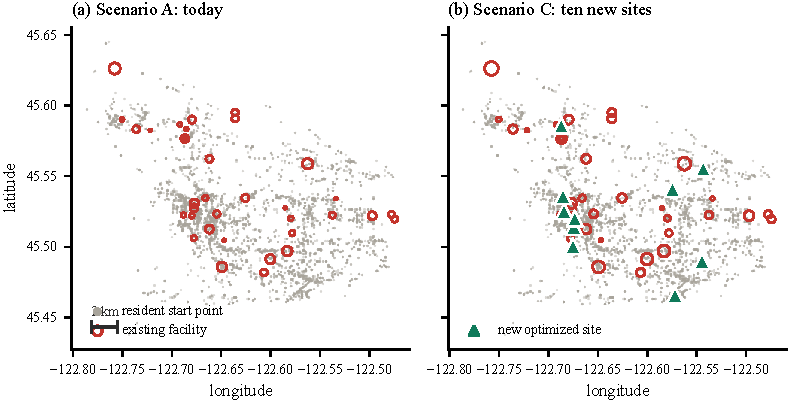
\includegraphics[width=\textwidth]{fig4_map}
\caption{Resident start points, in gray, against facility locations, sized by
capacity, in (a) today's system and (b) the better-placed scenario. In (a) the
existing facilities cluster away from much of the demand, while in (b) the ten
new sites are placed into the demand surface itself. The existing 36 facilities
are unmoved between panels; only the new capacity is placed.}
\label{fig:map}
\end{figure}

\subsection{Equity, and why the answer depends on the measure}
\label{sec:equity}

The second finding is one an analysis of totals cannot produce, because an
evaluation tracking only overall access would score scenario B as a
near-complete success. Table~\ref{tab:groups} reports access by group.

\begin{table}[t]
\caption{Percentage of each group reaching a shelter, seed 42.}
\label{tab:groups}
\begin{tabular}{p{3.8cm}p{1.5cm}p{1.4cm}p{1.4cm}p{1.4cm}}
\hline\noalign{\smallskip}
Group & Share (\%) & A (\%) & B (\%) & C (\%) \\
\noalign{\smallskip}\svhline\noalign{\smallskip}
Everyone & 100.0 & 30.1 & 91.6 & 96.0 \\
Walks without difficulty & 80.1 & 32.7 & 96.4 & 98.6 \\
Mobility limitation & 19.9 & 19.7 & 71.9 & 85.7 \\
Age 65 and over & 5.2 & 22.4 & 82.4 & 89.8 \\
COPD & 10.8 & 22.2 & 86.2 & 93.8 \\
Asthma & 14.8 & 29.2 & 90.6 & 95.7 \\
Chronic physical condition & 39.6 & 30.2 & 91.1 & 95.8 \\
\noalign{\smallskip}\hline
\end{tabular}
\end{table}

The direction of the equity result depends on how the gap is measured, so this
chapter reports three measures rather than one. Table~\ref{tab:gap} gives all
three for the comparison between residents who walk without difficulty and
residents with a mobility limitation. On a percentage-point scale, capacity
expansion widens the gap from 13.0 to 24.5, and better-placed capacity returns it
to 12.9. On a ratio scale the gap narrows at every step, from 1.66 to 1.34 to
1.15. Counting people rather than rates, the number of mobility-limited residents
left outside falls from 1,094 to 383 to 195.

\begin{table}[t]
\caption{The mobility gap on three measures. The last two rows are derived from
the group percentages in Table~\ref{tab:groups} applied to a population of 6,842,
and are rounded to the nearest resident and percentage point.}
\label{tab:gap}
\begin{tabular}{p{5.1cm}p{1.6cm}p{1.6cm}p{1.6cm}}
\hline\noalign{\smallskip}
Measure & A: today & B: more capacity & C: better placed \\
\noalign{\smallskip}\svhline\noalign{\smallskip}
Access, walks without difficulty (\%) & 32.7 & 96.4 & 98.6 \\
Access, mobility limitation (\%) & 19.7 & 71.9 & 85.7 \\
Difference in percentage points & 13.0 & 24.5 & 12.9 \\
Ratio of access rates & 1.66 & 1.34 & 1.15 \\
Mobility-limited residents left outside & 1,094 & 383 & 195 \\
Their share of all left outside (\%) & 23 & 66 & 72 \\
\noalign{\smallskip}\hline
\end{tabular}
\end{table}

These measures disagree because of a ceiling effect. At 96.4\% access in scenario
B, residents who walk without difficulty have almost no room left to improve, so
a percentage-point difference is compressed on one side of the comparison and not
the other. Reporting the percentage-point gap alone would present as widening
inequality what is, on other defensible scales, a narrowing one.
Section~\ref{sec:exposure} rejects a published parameter partly because the same
data yield different values depending on which scale is chosen. The same standard
applies to my own results.

Three statements survive every measure, and they are the equity findings this
chapter claims. First, every scenario improves absolute access for residents with
mobility limitations, from 19.7\% to 71.9\% to 85.7\%. Capacity expansion is not
harmful to this group; it helps them substantially. Second, residents with
mobility limitations remain the worst-served group under every scenario and are
over-represented among those still outside under every scenario. They are 19.9\%
of the population but 23\% of the residents left outside today, 66\% under
capacity expansion, and 72\% under better-placed capacity. As the system improves
in aggregate, the people who remain outside are increasingly the people who
cannot walk fast. This follows directly from first-come-first-served admission,
discussed in Sect.~\ref{sec:limitations}. Third, better-placed capacity closes
more of the remaining shortfall for this group than capacity alone: between B and
C, access for mobility-limited residents rises 13.8 percentage points against 2.2
for everyone else, and the ratio falls from 1.34 to 1.15. The gap is narrowed,
not closed; 14.3\% of residents with mobility limitations remain outside in
scenario C.

The same broad pattern holds for residents aged 65 and over, whose access moves
from 22.4\% to 82.4\% to 89.8\%, and for residents with COPD, from 22.2\% to
86.2\% to 93.8\%. Asthma shows almost no access penalty while COPD shows a large
one. This asymmetry follows from the available evidence rather than from an
oversight. In this model a diagnosis can affect an outcome only by affecting
walking speed, because a diagnosis is never a dose multiplier, and COPD carries a
published gait-speed decrement while asthma does not. Had I borrowed the COPD
estimate for asthma to make the treatment symmetric, I would have manufactured a
finding. The asymmetry is therefore evidence that the model is not inventing
effects.

The practical implication is narrow and testable. Any real expansion should be
evaluated on access broken down by group and reported on more than one scale, not
on totals and not on a single gap measure.

\subsection{Robustness}
\label{sec:robustness}

Across all 27 runs the largest seed-to-seed spread within a scenario is 11
residents, while the smallest difference between two scenarios at the same seed
is 306. The between-scenario signal is therefore roughly 28 times the
within-scenario noise, and no range overlaps between scenarios on any headline
metric, so the ordering A $<$ B $<$ C is not an artifact of any particular random
draw.

One detail falls out of the design as a free consistency check. The count of
residents who can reach no shelter at all is identical across all three scenarios
within each seed, at 16 at seed 42. These residents sit on street-graph
components containing no facility, so no amount of capacity and no re-placement
reaches them, and the number varies only with which residents were sampled. This
confirms the scenarios differ only in the way intended. It is not a check on
external accuracy.

\subsection{Calibration, and why none was possible}
\label{sec:calibration}

The model is not calibrated against observed shelter occupancy, because no
suitable record exists. Multnomah County did not publish occupancy figures for
its 2020 clean-air shelters in a form that could be compared against a
simulation, and I was unable to locate a systematic record from any other source.
This is a limitation of the available evidence rather than a modeling choice, and
it is the reason this chapter reports model-to-model comparisons rather than
predictions.

One assumption in particular means every access figure here should be read as an
upper bound. The model assumes that every resident knows the clean-air shelters
exist and knows where they are. In practice, information about temporary
emergency facilities reaches an unsheltered population unevenly, and a resident
who does not know a shelter exists will not walk toward it. Because awareness is
modeled as universal, the number of residents reaching shelter in each scenario
is the maximum the geography permits, not the number who would actually arrive.
This limitation applies identically to all three scenarios, so it does not affect
the comparison between them, which is what this chapter claims. It does affect
the absolute figures.

\section{Conclusion}
\label{sec:conclusion}

\subsection{Limitations}
\label{sec:limitations}

This study shows what the model can represent. It does not claim that the modeled
distances, exposure totals, or access rates match what a real expansion would
produce. Six limits matter most.

\textbf{The optimizer is evaluated on the demand it was fitted to.} All 27 runs
use identical resident starting coordinates, so the procedure that chooses the
ten new sites selects them to serve exactly the 2,981 campsite locations against
which scenario C is then measured. C's advantage over B is therefore an upper
bound on what the same procedure would achieve against a distribution of
campsites it had not seen.

\textbf{Several parameters are policy choices rather than measurements.} The
1.5$\times$ expansion factor, the choice of ten sites, and scenario B's uniform
3.06$\times$ scale-up were selected by me. The comparison establishes a
direction; the size of each effect would move with different values. The ten new
sites also average about 349 spaces each, larger than any facility in the real
inventory.

\textbf{Admission depends on arrival order.} Residents are served in shuffle
order rather than by need. This matters most in scenario A, where capacity binds
hardest, and it is the mechanism producing the concentration of mobility-limited
residents among the excluded that Sect.~\ref{sec:equity} reports. A needs-based
admission rule would likely change that result, so the equity findings should be
read as conditional on first-come-first-served admission.

\textbf{Every equity finding is downstream of the movement model,} because
walking speed is the only attribute permitted to affect an outcome. Those
distributions come from published meta-analyses rather than from local
observation, and no local validation of walking speeds among unsheltered
residents was possible within the scope of this project.

\textbf{Several known problems work against the conclusions rather than for
them,} and are stated for that reason. Ten day centers are excluded because none
publishes a capacity, yet during a daytime smoke episode they are plausibly the
most relevant clean-air spaces that exist, so scenario A understates present-day
daytime availability, and scenario A is the baseline. Every mobility-limited
resident is assigned the fastest of the published impaired-movement categories,
so the modeled mobility penalty is conservative. Two real facilities totaling
about 207 spaces are missing entirely.

\textbf{The inputs carry their own limits.} The PM$_{2.5}$ field is spatially
uniform, because with two in-county monitors any interpolation would manufacture
gradients the data cannot support; one consequence is that placement can help
only by reducing time outdoors, never by moving people into cleaner air. The
monitors are non-reference instruments that most likely understate true
concentrations during fresh wood smoke. Encampment locations are 2025 and 2026
complaint-driven reports used as a spatial proxy for 2020. Sex and mobility
distributions are 2019 data, and asthma and COPD prevalences are imported from a
Minnesota cohort because no local equivalent exists.

The project was also narrower in scope than originally planned. It was proposed
with five siting scenarios, projected-future smoke conditions, and a second
research question about weighting exposure by residents' relative risks. Three
scenarios are reported, all results use the measured 2020 event, and
Sect.~\ref{sec:exposure} explains why the weighting question could not be
answered. The three reported are the ones needed to separate a capacity failure
from a geography failure, which is the question that turned out to have an
answer.

\subsection{Summary and Next Steps}
\label{sec:summary}

This study asked a direct question: for a fixed total capacity, does placement
change how many unsheltered residents reach a clean-air shelter, and does it
change which residents reach one?

The answer to the first is yes. The present system shelters 30.1\% of residents.
Raising capacity to match the population shelters 91.6\% and still refuses 562
people while holding exactly one space per person. Spending the identical
capacity on ten better-placed sites shelters 96.0\% and cuts refusals to 256. The
ordering held across nine random seeds with no overlap between scenarios on any
headline metric.

The answer to the second is yes, with a caveat about measurement that matters as
much as the result. On a percentage-point scale, capacity expansion widens the
mobility gap and better-placed capacity closes it; on a ratio scale, both narrow
it. What holds regardless of scale is that residents with mobility limitations
remain the worst-served group throughout and make up a growing share of those
still outside as the system improves, rising from 23\% of the excluded today to
72\% under the best scenario modeled, against a 19.9\% population share.

If Multnomah County can add clean-air shelter capacity, that dominates every
other intervention modeled here. But the second finding is the one with no budget
attached. Once capacity is adequate in aggregate, where the marginal capacity
sits determines whether it is usable, and the same 6,842 spaces more than halve
refusals depending only on placement. A capacity expansion evaluated on aggregate
access would look like a success while the percentage-point gap nearly doubled.

Four extensions would improve the model most. A model of awareness is the most
valuable single addition: the chapter assumes every resident knows the shelters
exist, and that assumption is what makes each access figure an upper bound.
Giving each resident a probability of knowing, swept across a range, would turn
each figure from a single upper bound into an interval and would give the model a
parameter that could be fitted if occupancy data ever becomes available. Second,
an inequality measure computed over the full distribution of exposure, such as a
Gini coefficient, would give a fourth equity statistic free of the ceiling effect
described in Sect.~\ref{sec:equity}. Third, an order-independent admission
procedure would remove the shuffle-order dependence and let a needs-based triage
rule be compared against first-come-first-served, so the equity result could be
challenged on policy grounds rather than only on geometry. Fourth, the placement
procedure should be fitted on one set of campsite locations and evaluated on
another.

The approach generalizes beyond smoke. The same structure --- a hazard varying
over time, a population with heterogeneous mobility at real locations, and a
capacitated set of refuges on a real network --- applies to extreme-heat cooling
centers, warming shelters, and emergency distribution points. The finding that
capacity added at existing sites is claimed first by whoever walks fastest is a
hypothesis those settings could test.

\begin{acknowledgement}
This work was completed through the National Science Foundation Research
Experiences for Undergraduates program, Computational Modeling Serving Portland,
hosted by Portland State University under Grant No.
\authornote{[NSF award number to be inserted]}. I thank Prof. Christof Teuscher
for his mentorship and guidance throughout the program.

I directed the research, made all research decisions, and wrote the manuscript.
Claude (Anthropic) assisted with coding, with data-acquisition and analysis
scripting, with verification tooling, with drafting documentation, and with the
citation audit reported in Sect.~\ref{sec:exposure}, which I then verified
against the original publisher records. I reviewed, revised, and approved all
outputs, and I take full responsibility for the final text and for every number
in it.
\end{acknowledgement}

\noindent\textbf{Code and data availability.} The full simulation source,
analysis scripts, input data, configuration files, and all 27 run manifests are
available at \url{https://github.com/fxa28196/REU} under the MIT License. Every
result was produced from a clean working tree. Each run manifest records its git
commit, random seed, Java and Repast versions, every parameter value, and a
SHA-256 checksum for every input file. The reported results use seeds 42 through
50, with seed 42 as the reported run. The EPA air-quality data and the City of
Portland campsite reports are public and their retrieval scripts are included.
The street centerline file is redistributed as received; its original release
version and license could not be recovered, so the repository's license file
states its terms as unverified rather than relicensing it.

\begin{thebibliography}{99}

\bibitem{atkinson2013}
Richard W. Atkinson, Iain M. Carey, Andrew J. Kent, Tjeerd P. van Staa, H. Ross
Anderson, and Derek G. Cook. Long-term exposure to outdoor air pollution and
incidence of cardiovascular diseases. \emph{Epidemiology}, 24(1):44--53, 2013.

\bibitem{bohannon1997}
Richard W. Bohannon. Comfortable and maximum walking speed of adults aged 20--79
years: reference values and determinants. \emph{Age and Ageing}, 26(1):15--19,
1997.

\bibitem{bohannon2011}
Richard W. Bohannon and A. Williams Andrews. Normal walking speed: a descriptive
meta-analysis. \emph{Physiotherapy}, 97(3):182--189, 2011.

\bibitem{boyce1999}
Karen E. Boyce, T. J. Shields, and G. W. H. Silcock. Toward the characterization
of building occupancies for fire safety engineering: capabilities of disabled
people moving horizontally. \emph{Fire Technology}, 35(1):51--67, 1999.

\bibitem{brown2017}
Rebecca T. Brown, Kaveh Hemati, Elise D. Riley, Christopher T. Lee, Claudia
Ponath, Lina Tieu, David Guzman, and Margot B. Kushel. Geriatric conditions in a
population-based sample of older homeless adults. \emph{The Gerontologist},
57(4):757--766, 2017.

\bibitem{buekers2024}
Joren Buekers, Laura Delgado-Ortiz, Dimitrios Megaritis, Ashley Polhemus, Sofie
Breuls, Sara C. Buttery, Nikolaos Chynkiamis, Heleen Demeyer, Elena
Gimeno-Santos, Emily Hume, Sarah Koch, Parris Williams, Marieke Wuyts, Nicholas
S. Hopkinson, Ioannis Vogiatzis, Thierry Troosters, Anja Frei, and Judith
Garcia-Aymerich. Gait differences between COPD and healthy controls: systematic
review and meta-analysis. \emph{European Respiratory Review}, 33(172):230253,
2024.

\bibitem{portlandcampsites}
City of Portland. Impact Reduction Program campsite reports (open data). ArcGIS
feature service, 2026. Retrieved 24 July 2026.

\bibitem{portlandsrv}
City of Portland. Safe Rest Villages, 2026. Retrieved 24 July 2026.

\bibitem{deflorio2019}
Stephanie DeFlorio-Barker, James Crooks, Jeanette Reyes, and Ana G. Rappold.
Cardiopulmonary effects of fine particulate matter exposure among older adults,
during wildfire and non-wildfire periods, in the United States 2008--2010.
\emph{Environmental Health Perspectives}, 127(3):037006, 2019.

\bibitem{devries2017}
Rebecca DeVries, David Kriebel, and Susan Sama. Outdoor air pollution and
COPD-related emergency department visits, hospital admissions, and mortality: a
meta-analysis. \emph{COPD: Journal of Chronic Obstructive Pulmonary Disease},
14(1):113--121, 2017.

\bibitem{di2017}
Qian Di, Yan Wang, Antonella Zanobetti, Yun Wang, Petros Koutrakis, Christine
Choirat, Francesca Dominici, and Joel D. Schwartz. Air pollution and mortality in
the Medicare population. \emph{New England Journal of Medicine},
376(26):2513--2522, 2017.

\bibitem{dijkstra1959}
Edsger W. Dijkstra. A note on two problems in connexion with graphs.
\emph{Numerische Mathematik}, 1(1):269--271, 1959.

\bibitem{fazel2014}
Seena Fazel, John R. Geddes, and Margot Kushel. The health of homeless people in
high-income countries: descriptive epidemiology, health consequences, and
clinical and policy recommendations. \emph{The Lancet}, 384(9953):1529--1540,
2014.

\bibitem{karney2013}
Charles F. F. Karney. Algorithms for geodesics. \emph{Journal of Geodesy},
87(1):43--55, 2013.

\bibitem{multcohsd}
Multnomah County Health and Human Services. List of shelters, 2026. Retrieved 24
July 2026.

\bibitem{north2013}
Michael J. North, Nicholson T. Collier, Jonathan Ozik, Eric R. Tatara, Charles M.
Macal, Mark Bragen, and Pamela Sydelko. Complex adaptive systems modeling with
Repast Simphony. \emph{Complex Adaptive Systems Modeling}, 1(1):3, 2013.

\bibitem{deq2023}
Oregon Department of Environmental Quality. Wildfire smoke trends and the air
quality index. Technical report, Oregon Department of Environmental Quality, Air
Quality Monitoring, Hillsboro, Oregon, 2023. 2023 edition.

\bibitem{psupit2025}
Portland State University Homelessness Research and Action Collaborative. 2025
Tri-County Point-in-Time count findings summary report. Technical report,
Portland State University, 2025.

\bibitem{reid2016}
Colleen E. Reid, Michael Brauer, Fay H. Johnston, Michael Jerrett, John R.
Balmes, and Catherine T. Elliott. Critical review of health impacts of wildfire
smoke exposure. \emph{Environmental Health Perspectives}, 124(9):1334--1343,
2016.

\bibitem{siam2022}
Md Rakibul Karim Siam, Haizhong Wang, Michael K. Lindell, Chen Chen, Eleni I.
Vlahogianni, and Kay Axhausen. An interdisciplinary agent-based multimodal
wildfire evacuation model: critical decisions and life safety.
\emph{Transportation Research Part D: Transport and Environment}, 103:103147,
2022.

\bibitem{ucsf2023}
University of California, San Francisco Benioff Homelessness and Housing
Initiative. Toward a new understanding: the California statewide study of people
experiencing homelessness. Technical report, University of California, San
Francisco, 2023.

\bibitem{epaefh2011}
U.S. Environmental Protection Agency. Exposure factors handbook: 2011 edition,
chapter 6: Inhalation rates. Technical Report EPA/600/R-09/052F, U.S.
Environmental Protection Agency, National Center for Environmental Assessment,
2011.

\bibitem{epaaqs2020}
U.S. Environmental Protection Agency. Air Quality System (AQS) pre-generated data
files: hourly fine particulate matter, parameter 88502, 2020. Retrieved 24 July
2026.

\bibitem{epaaqi2024}
U.S. Environmental Protection Agency. Technical assistance document for the
reporting of daily air quality: the Air Quality Index (AQI). Technical report,
U.S. Environmental Protection Agency, Office of Air Quality Planning and
Standards, Research Triangle Park, North Carolina, 2024.

\bibitem{zellmer2025}
Lucas Zellmer, Renee Van Siclen, Peter Bodurtha, Paul E. Drawz, Stephen C.
Waring, Alanna M. Chamberlain, Behnam Sabayan, Steven G. Johnson, Karen Margolis,
Rebecca Rossom, Katherine Diaz Vickery, and Tyler N. A. Winkelman. Estimating
health condition prevalence among a statewide cohort with recent homelessness or
incarceration. \emph{Journal of General Internal Medicine}, 2025.

\end{thebibliography}

\end{document}
